%!TEX root = project.tex

\chapter{Technology Review}
About seven to ten pages.
\begin{itemize}
    \item Describe each of the technologies you used at a conceptual level. Standards, Database Model (e.g. MongoDB, CouchDB), XMl, WSDL, JSON, JAXP.
    \item Use references (IEEE format, e.g. [1]), Books, Papers, URLs (timestamp) – sources should be authoritative.
\end{itemize}

\begin{figure}[H]
    \centering
    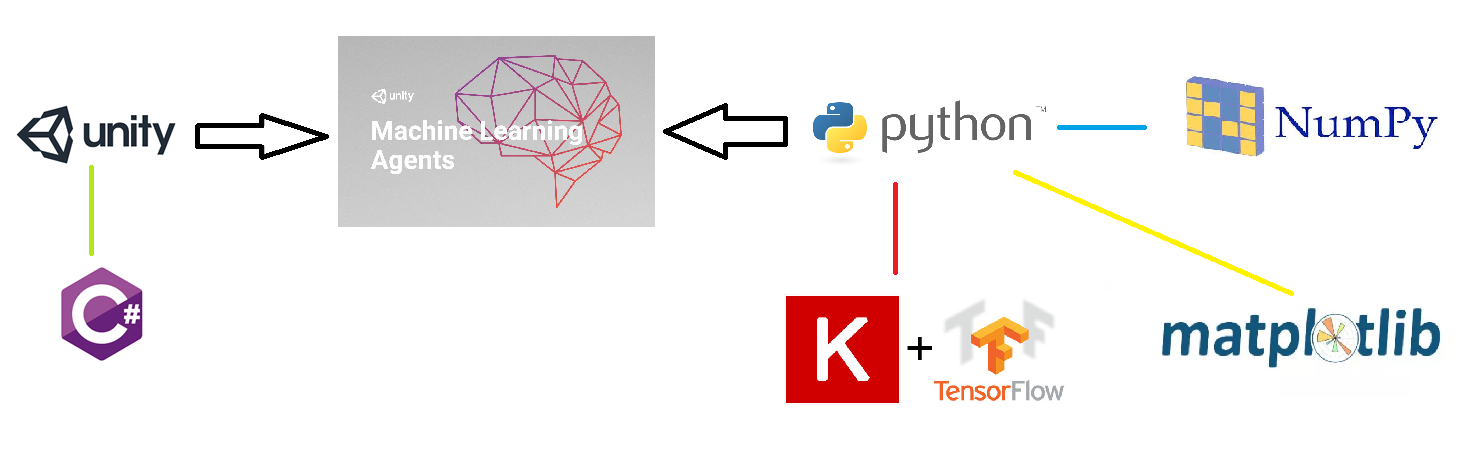
\includegraphics[width=130mm, height=35mm]{img/TechUsed.png}
    \caption{Technologies used}
    \label{fig:sd4}
\end{figure}

\section{History of AI}
The initial idea of artificial intelligence was first brought around during the second world war where Alan Turing and his team developed the Bombe machine, a device capable of deciphering messages from the enigma machine. Turing stated that a machine that could converse with a human, without the human knowing that they were conversing with a machine could be said to be “Intelligent”.  With this, the foundations for artificial intelligence was created. 

John McCarthy is said to be the “father” of Artificial Intelligence, coining the term in the year 1955. He invented his own programming language, LISP which became the programming language of choice for AI development. 

Despite AI development being around for so long, research fell subject to what was known as “AI Winters”. During these phases funding for development of AI was reduced due to lack of processing power and interest fell short. With the turn of the century, research started to pick up again due to the advancements in hardware and the processing power of machines.

\section{Machine Learning}
Machine learning (ML) is an application of artificial intelligence (AI) that provides systems the ability to automatically learn and improve from experience without being explicitly programmed. Machine learning focuses on the development of computer programs that can access data and use it learn for themselves.

One of the current trends in modern day software development is the exploration into the world of Artificial intelligence.
With the recent boom of Artificial Intelligence and Machine learning, we thought it would be a good idea to jump onto the bandwagon and see what it was all about.
In this paper we will describe in detail our process of creating an unity environment with the goal of teaching an agent how to play soccer, the challenges encountered throughout and the research done into the areas of Machine Learning and the Unity environment.  We will then discuss how we implemented this idea with ideas acquired from our research. We will then discuss our results, what we learned and how we could possible improve on in the future with further research.

\section{Neural Networks}
Neural network, a computer program that operates in a manner inspired by the natural neural network in the brain. The objective of such artificial neural networks is to perform such cognitive functions as problem solving and machine learning.
\section{Unity}
Unity is a cross-platform real-time engine developed by Unity Technologies. The engine can be used to create both three-dimensional and two-dimensional games as well as simulations for its many platforms.
\section{Python}
Python is an interpreted, object-oriented, high-level programming language with dynamic semantics. Its high-level built in data structures, combined with dynamic typing and dynamic binding, make it very attractive for Rapid Application Development, as well as for use as a scripting or glue language to connect existing components together. Python's simple, easy to learn syntax emphasizes readability and therefore reduces the cost of program maintenance. 

\section{Jupyter Notebook}
Notebooks
Through the use of the Jupyter notebook, we could develop our AI through python while also documenting it in a nice style with the use of the Markdown option. This provided a clear user-friendly experience when running the python code through the notebook with in depth explanations of what our code does. The Jupyter notebook app is a server to client application that allows users to create notebook documents and run then via the web browser. This app can be run on a local desktop without the requirement of internet access through the command line. There is also a similar version of this web app called Jupyter Lab. This version of the web app grants the user a more IDE-like experience, allowing the user to have many tabs in the same window. With our development we went with using the Jupyter Lab version over the Jupyter Notebook version as we found it more useful due to the number of notebooks we would be developing and the GUI similar to an IDE made it more comfortable to work in. 

To open the Jupyter notebook version of the web application, enter the following into the command line
\begin{minted}{console}	
	Jupyter notebook 
\end{minted}
To open the Jupyter lab version of the web application, enter the following into the command line
\begin{minted}{console}
	Jupyter lab 
\end{minted}

%Look at this again - Ryan
\subsection{How it works}
The notebooks are broken up into individual cells. Each individual cell can be specified into three different types of syntax: Markdown, Python and Raw text. Below is an example of both a Markdown and a python cell taken from our project before they are executed.

\begin{figure}[H]
    \centering
    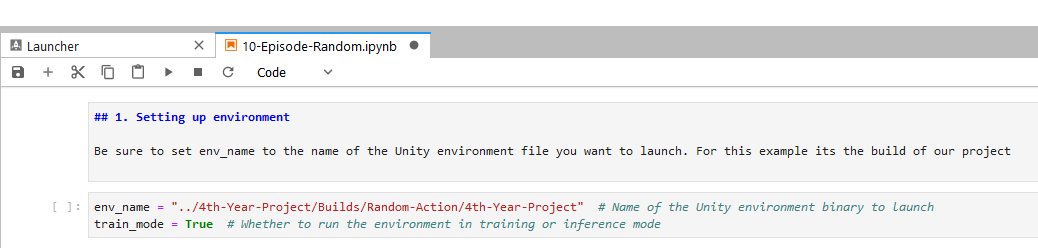
\includegraphics[width=115mm, height=30mm]{img/Notebook1.PNG}
    \caption{Notebook cells before execution}
    \label{fig:sd4}
\end{figure}

\begin{flushleft}
As you can see the first cell block contains the markdown syntax and the second cell containing python syntax before they have been executed.
\end{flushleft}

\begin{figure}[H]
    \centering
    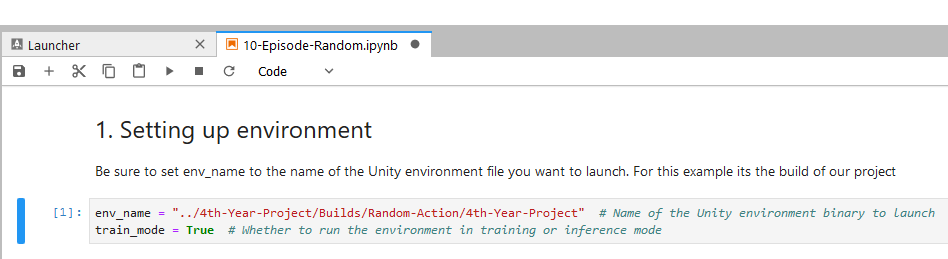
\includegraphics[width=115mm, height=30mm]{img/Notebook2.PNG}
    \caption{Notebook cells after execution}
    \label{fig:sd4}
\end{figure}

\begin{flushleft}
In this image we see both cells after being executed. The number "1" to the left of the cell indicates that this has finished running and its the first python cell that has been executed in the notebook. 
\end{flushleft}

%end

\section{Technologies Review}
This chapter will discuss in detail the technologies that we utilised in the project. It will also provide examples of the research we did into the different types of possible technologies. It will also highlight the rationale behind the decisions we made to use certain technologies over others.

\section{Game Engines}
In this section, we will discuss the possible game engines we can use to run our environment in. We don't want to try use actual hardware and would prefer to run our environment in a game engine.

\subsection{Unity}
Unity is a real-time game engine developed by Unity Technologies and released back in June of 2005. Originally designed as an OSX-exclusive game engine, the software has been developed upon and extended to support a host of other platforms also~\cite{unityWebsite}. Unity has made a name for itself, making game development accessible to everyone, as shown by the sheer amount of indie game developers using Unity as there main game engine tool.

\subsubsection{Why use Unity}
The main pull Unity has over other game engines is it's ease of use, the software has been designed to make it easy to design games from the ground up, with easy to understand UI and an overall aim to create functional, smart, and sometimes simple games, rather than complex games with high quality graphics. Also the fact that the software is free to download and use is a big plus~\cite{JoshPetty}.

\subsection{Unreal Engine}
Unreal Engine was developed alongside it's debut title "Unreal" in 1998 by Epic Games. The game engine has kept a reputation of it being a high end piece of software, both due to it's price plans, and it's ability to generate incredible graphics~\cite{unrealEngine4}.

\subsubsection{Why use Unreal}
The software has had some problems in the past with it's steep learning curve. Certainly not a beginners piece of software, however if someone who has had previous experience with coding and other 3d programs is looking to create a highly detailed expansive game, they need look no further than Unreal Engine~\cite{unrealEngine4Overview}.

\subsection{Our decision}
We decided to use Unity over Unreal Engine, firstly because of the learning curve. We had the opportunity to use Unity previously in a module, so we all had a slight bit of experience. Also the fact Unity is completely free, whereas Unreal Engine requires a payment plan to be set up, was what finally sold us on using Unity.

\section{Neural Network Languages}
In this section we will discuss the different languages we reviewed to write our neural network in. The following programming languages have all been noted as strong languages for neural network design.

\subsection{Python}
Created by Guido van Rossum, Python is a high level, general purpose programming language first released in 1991. Pythons design philosophy emphasizes code readability, meaning the language utilises a significant amount of white space~\cite{whatIsPython}. The language supports multiple programming paradigms, so programs written procedurally will work just as well as an object oriented program design~\cite{pedregosa2011scikit}.

\subsubsection{Why Python} 
Simplicity is a major factor when talking about neural network design, so having a language that's easy to understand, as well as the fact that python has an extremely large library of useful frameworks to utilise makes it a very strong choice~\cite{whatIsPythonForBeginners}.

\subsection{R - Programming language}
R is a programming language and software environment used for statistical computing, and is great for producing informative graphics and data mining~\cite{rAbout}. Originally introduced back in 1993, the language has stuck around due to it's presence as a truly general purpose programming language~\cite{hornik2009open}.

\subsubsection{Why R}
Although R doesn't originally apear to be a language that would suit neural network design, the sheer amount of libraries that R boasts, including RODBC, Gmodels, and Tm, which are all used in the field of machine learning, means the language actually has a strong case for being the correct one to use~\cite{rIntroAndBasics}.

\subsection{Lisp}
Lisp is a family of programming languages, originally specified way back in 1958. It is the second oldest high level programming language that is still in widespread use today. John McCarthy, the inventor of the language, is actually known as the father of Artificial Intelligence, and many of the languages features have been implemented and migrated over into more modern programming languages~\cite{LISPIntro}.

\subsubsection{Why Lisp}
Apart from it's inventor holding the title of the father of AI, Lisp actually became the favoured language for AI development and research shortly after it's introduction~\cite{LISPTut}.

\subsection{Our decision}
We decided to use Python as our language to build the neural network in due to the fact that the language is currently considered to be on top when it comes to AI development. Even though R and Lisp both were strong candidates for what language to use, the fact that Python is designed to be so simplistic and easy to understand made it the best choice for us, as we would need to be able to get our heads around the inner workings of neural networks quickly.

\section{Connector Software}
In this section we will discuss the possible ways to connect the neural network code to the game engine environment.

\subsection{Jupyter Notebooks}
The Jupyter Notebook App is a server-client application that allows the editing and running of notebook documents via a web browser~\cite{jupyterSite}. Notebook documents are produced by the App and can contain both computer code as well as rich text elements. These documents acts as an executable which can run whatever code they consist of~\cite{jupyterDocs}.

\subsubsection{Why Jupyter Notebooks}
We have had previous experience with notebooks, using them in a previous module, so we already have an understanding of their inner workings. We also found plenty of examples of other people connecting game engine environments to  external code. Having a previous understanding of the ins and outs of these notebook documents will be a great advantage to using notebooks as a connector between the environment and external code~\cite{MikeDriscoll}.

\subsection{Transmission Control Protocol connection}
TCP is one of the main protocols of the Internet protocol suite~\cite{TCP}. 
TCP provides a reliable, ordered, and error-checked delivery of a stream of bytes between applications communicating via an IP network~\cite{TCPsdx}. 

\subsubsection{Why Transmission Control Protocol}
A TCP connection has been attempted to connect a game engine environment to external neural network code by others~\cite{UnityTCP}. We found some examples of other attempts, with some positive results. The bonus to using a TCP connection would be the fact that literally anything could be passed between the environment and the external code. Json objects could be passed back and forth meaning any input needed for the neural network, and subsequent output, could all be passed back and forth with ease, once a connection between the two had been established.

%new
ML-Agents
ML-Agents is a new open-source Unity plugin designed by Unity themselves, which aims to provide an expansive toolkit within the Unity environment to help with the development of machine learning. The software enables games and simulations to serve as environments for training AI agents. 

Why ML-Agents
Using ML_Agents is the perfect choice for us, since we have decided to use the Unity engine to develop our 3d environment in. The documentation for ML-Agents shows us exactly how we could use this plugin to aid us in creating agents in our Unity environment.






IronPython
IronPython is an open-source implementation of Python. The implementation uses the .NET framework, as well as the entire suite Python libraries. The class library also contains language interoperability, meaning each language can use code written in another language.

Why IronPython
IronPython having the ability to use the .NET framework could work well for us connecting our environment to our external code. The .NET framework’s expansive class library has plenty of useful resources that we could utilise.









Neural network libraries
In this section we will discuss the possible neural network libraries we could utilise in our project. Using a machine learning library could be very useful for developing our neural network and ML models, as well as offer easier debugging options for testing.

TensorFlow
TensorFlow is an end-to-end open source platform for machine learning. Its flexible ecosystem of tools, libraries and resources allow for easy development and deployment of ML powered applications.

Why Tensorflow
Tensorflow is a very well-known platform for ML powered applications. Having a platform that we can use to train models easily could be very useful when designing our own models.

Sony’s neural network libraries
Neural Network Libraries by Sony is an open source software aiming to make research, development and implementation of neural networks more efficient.

Why Sony’s neural network libraries
Having a fully optimised library of ML related code could be extremely useful when designing and implementing our own neural network. Although the software isn’t as widespread as TensorFlow, it could be better suited for our needs.

Our Decision
We decided to have TenserFlow as our go to neural network library for two main reasons. Firstly, Sony’s neural network libraries aren’t as widely used as TenserFlow, meaning examples and other documentation is harder to come by. And secondly, we started a module in our course which utilises TensorFlow, meaning we are already starting to learn what the libraries can be used for and how we could adapt it into our own project if needed.

Unity Test Tools 
Unity Test Tools is a test framework for any games and interactive content made in Unity. The framework is built to feel like a natural extension of the Unity Editor, so everything should be intuitive to anyone with experience using the Editor itself.


Why Unity Test Tools
The fact that these tools are easily accessible from the Unity asset store, as well as the fact they were designed by the Unity developers themselves, means they will work perfectly with the environment we build.

Our decision
We decided the use of the Unity Test Tools would actually not be very useful, since the fact that the majority of the work being performed will be external to the Unity environment. Having test data from just the environment itself isn’t necessary for the type of project we are aiming to create.





%new


Docker
Docker is a tool designed to help create, deploy and run applications. The tool uses containers to package all the necessary components, including libraries and other dependencies, into one single package. This means that any developer can rest assured the application will run on any machine.

Why Docker
Using Docker would allow us to focus on the coding and development of the project, without having to worry about the system that our application will ultimately be running on. Having everything packaged together would help with the final deployment of the project, guaranteeing the entire project would run on any system without a shadow of a doubt.

Our Decision
In the end we decided not to work using Docker, even though the tool is very intriguing and would be a major help running the project in the later stages, through some research we found complaints that the containers can be subject to performance overhead, and with our project, running the simulations at a consistent rate is very important. Also our project consists of multiple possible scenes and scenarios to run from multiple different notebooks, meaning that using Docker wouldn’t allow the final user to run whichever scenario they wishes, as Docker uses a single command to run it’s packages content, and doesn’t offer the ability to run multiple different parts of its package independently for the final user.


Anaconda
Anaconda is a free and open-source distribution of Python and R programming languages for scientific computing, including machine learning applications. The distribution aims to simplify package management and deployment, offering over 1400 data-science packages.
Why Anaconda
Anaconda would offer an easy and efficient way for us to gather the necessary packages for our machine learning needs. If we decide to use either Python or R as our programming language of choice, then Anaconda may be a great option for us.

Our Decision
We decided to utilise Anaconda since we are using Python to build the neural network side to our project. The distribution includes matplotlib, numpy, and keras, which we aim to also use in our project, meaning Anaconda will be very helpful in installing these packages.



%new
